%%==========================================================================
\section{Experiments}
\label{sec:experiments}

We have used synthetically generated data as well as real captured data to evaluate the SuperMatching algorithm.
To demonstrate that the SuperMatching algorithm is general (independent of feature descriptors), several descriptors have been used.
For the input shapes without color information, slippage features~\cite{Bokeloh08} were employed.
For 3D coloured shapes, both SIFT and slippage features were used.
We used third-order matching in our experiments, and note it would be simple to use higher order.
%%%RRM But presumably slower?
%For greater than third higher-order, it is easy to replace the potential by relevant polygonal definitions.

%-------------------------------------------------------------------------
\subsection{3D rigid shapes scans}
\label{subsec:3DRigid}

Firstly, we used SuperMatching to pairwisely align 3D rigid shape scans.
The rigid transforms can be computed from the three compatible matching feature points.
The transform which brings the most data points within a threshold of a point in the model is chosen as the optimal aligning transform~\cite{Huttenlocher90}.
As discussed in~\cite{Gelfand05}, such a voting scheme is guaranteed to find the optimal alignment between the pairwise scans and is independent of the initial pose of the input scans.
Figure~\ref{fig:3DPair} shows two registration examples of articulated model, the right is the failure case by~\cite{Aiger08}.

\begin{figure}[htb]
\centering
  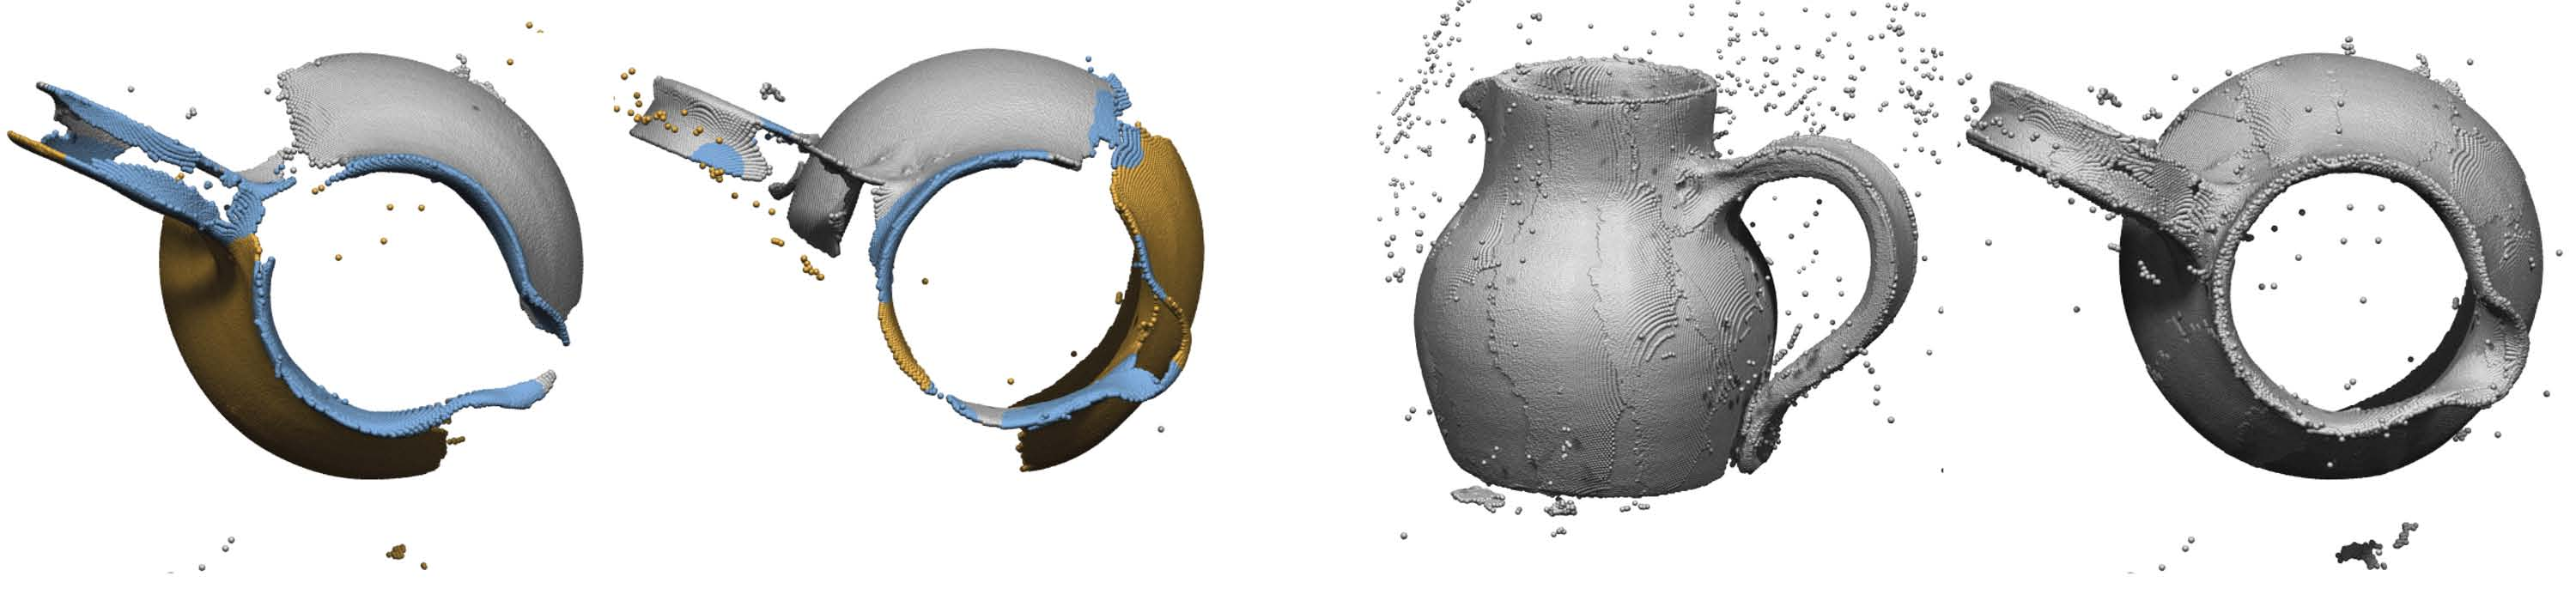
\includegraphics[width=0.99\linewidth]{figures/rigidCMP.jpg}
  \caption{Pairwise alignment of xx. The right is the result from [Aiger et al. 2008]. \cz{On the coming :)}}
\label{fig:3DPair}
\end{figure}

In the following, we extended the SuperMatching to build a complete model from a set of scans from different viewpoints.
For the multiple scans, the third-order matching is first performed between two consecutive scans.
After the initial pairwise matching, the alignment is refined by the iterative closest point (ICP) algorithm following~\cite{Gelfand05}.
Figure~\ref{fig:3DRigid} illustrates the approach.
Above, a sheep's head is scanned from multiple viewpoints. Below, matching is used to align 10 scans which are then merged to produce a single shape.
Pairs of consecutive scans, linked by dark segments, are matched using the SuperMatching algorithm.

\begin{figure}[h]
\centering
  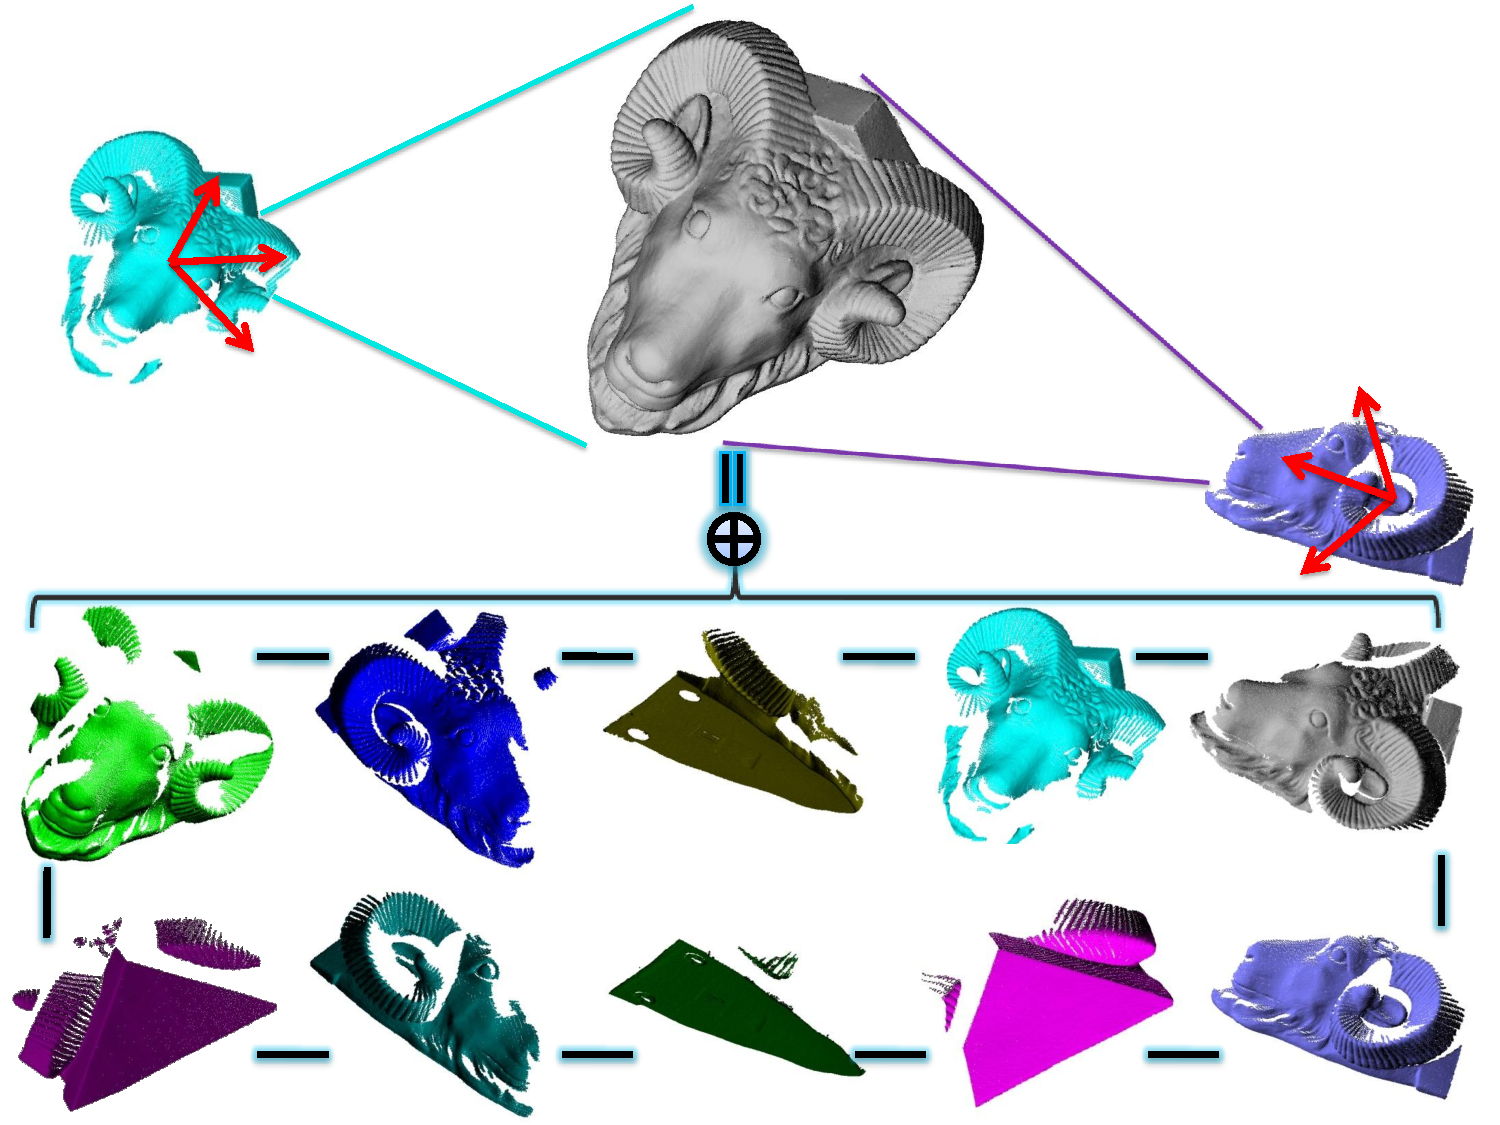
\includegraphics[width=0.99\linewidth]{figures/3DRigid.pdf}
  \caption{Alignment of several sheep head scans from different viewpoints. 
  Above: scans are captured from different viewpoints. Below: the final shape is formed from 10 aligned scans, the dark segments imply where the pairwise matching works.}
\label{fig:3DRigid}
\end{figure}

%%%RRM Actually, there are some datasets out there with known transofrmations
%%%RRM between them. We could try to show we can estimate the transformations
%%%RRM more accurately than other methods.
%%%RRM See for example the dataset used in
%%%RRM http://ralph.cs.cf.ac.uk/papers/Geometry/crf.pdf

%-------------------------------------------------------------------------
\subsection{3D depth scans with color information}
\label{subsec:3dColored}

Complementary to the evaluation presented above,
we also provide a real-world noisy example demonstration of SuperMatching. 
In this case, real world data with surface color information was captured using a Kinect camera~\cite{Kinect12}, 
and both SIFT and slippage features were used as a basis for SuperMatching,
which resulted in robust matches without significant outliers, as illustrated in Figure~\ref{fig:3DReal}.
The example also demonstrates that the SuperMatching is general, i.e., independent of feature descriptors.

\begin{figure}[h]
\centering
  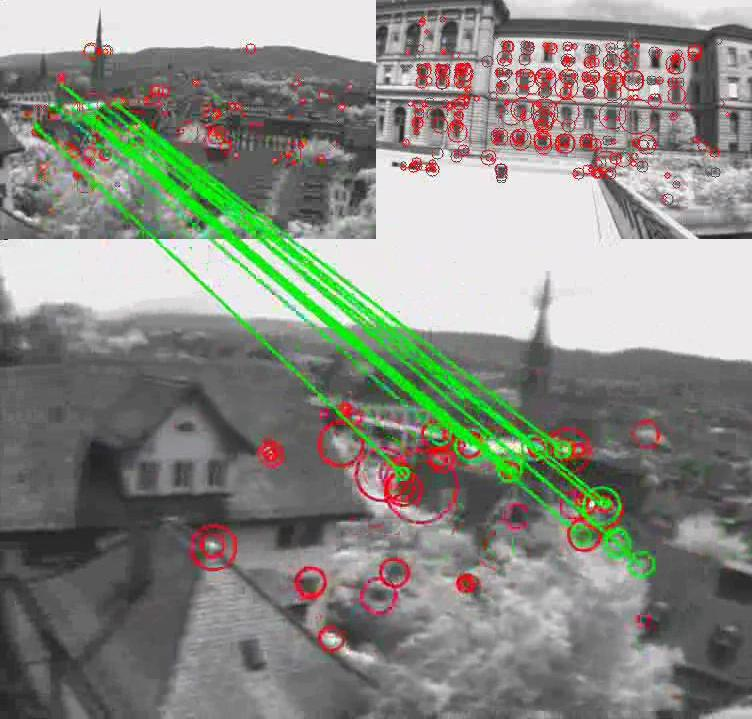
\includegraphics[width=0.9\linewidth]{figures/3DReal.jpg}
  \caption{3D real depth scans with color information, captured using Kinect.
  Above: two given different local pre-scans.  Below: a single scan.
  Matching points are connected by green lines.}
\label{fig:3DReal}
%%%RRM I dont really understand this result. I though the kinect scanned
%%%RRM nearby objects yet this shows pictures of trees and buildings a long distance away
%%%RRM Also, I dont see the point of the top right image here. It shows nothing
%%%RRM about matching.
\end{figure}

%-------------------------------------------------------------------------
\subsection{3D articulated shape synthetic data}
\label{subsec:3darticulated}

Thirdly, we present another application, registration of (approximately) articulated shapes. Such problems are common in dynamic range scanning.
Given a sequence of range scans of a moving articulated subject, our method automatically registers all data to produce a complete 3D shape.
Note that, unlike many other methods, our method does not need any of manual segmentation, user specified markers, or a prior template.
While the problem of non-rigid registration of deformable shapes is ill-posed and no algorithm is applicable to all scenarios,
we believe that our approach pushes the limits of what can be achieved with minimal prior information, and is robust to partial data with holes.

For the pairwise articulated shape registration, 
although the partial scans have missing data and their poses are different, SuperMatching still produces accurate matching.
Correspondences between slippage feature points are established by SuperMatching; 
these permit robust registration of scans by computing piecewise rigid transformations.
These transformations are propagated from the slippage feature points to the entire set of points in each scan using nearest neighbor interpolation.
Figure~\ref{fig:3DRobot} shows two registration examples of articulated model, the right is the failure case by~\cite{Chang09}.

\begin{figure}[h]
\centering
  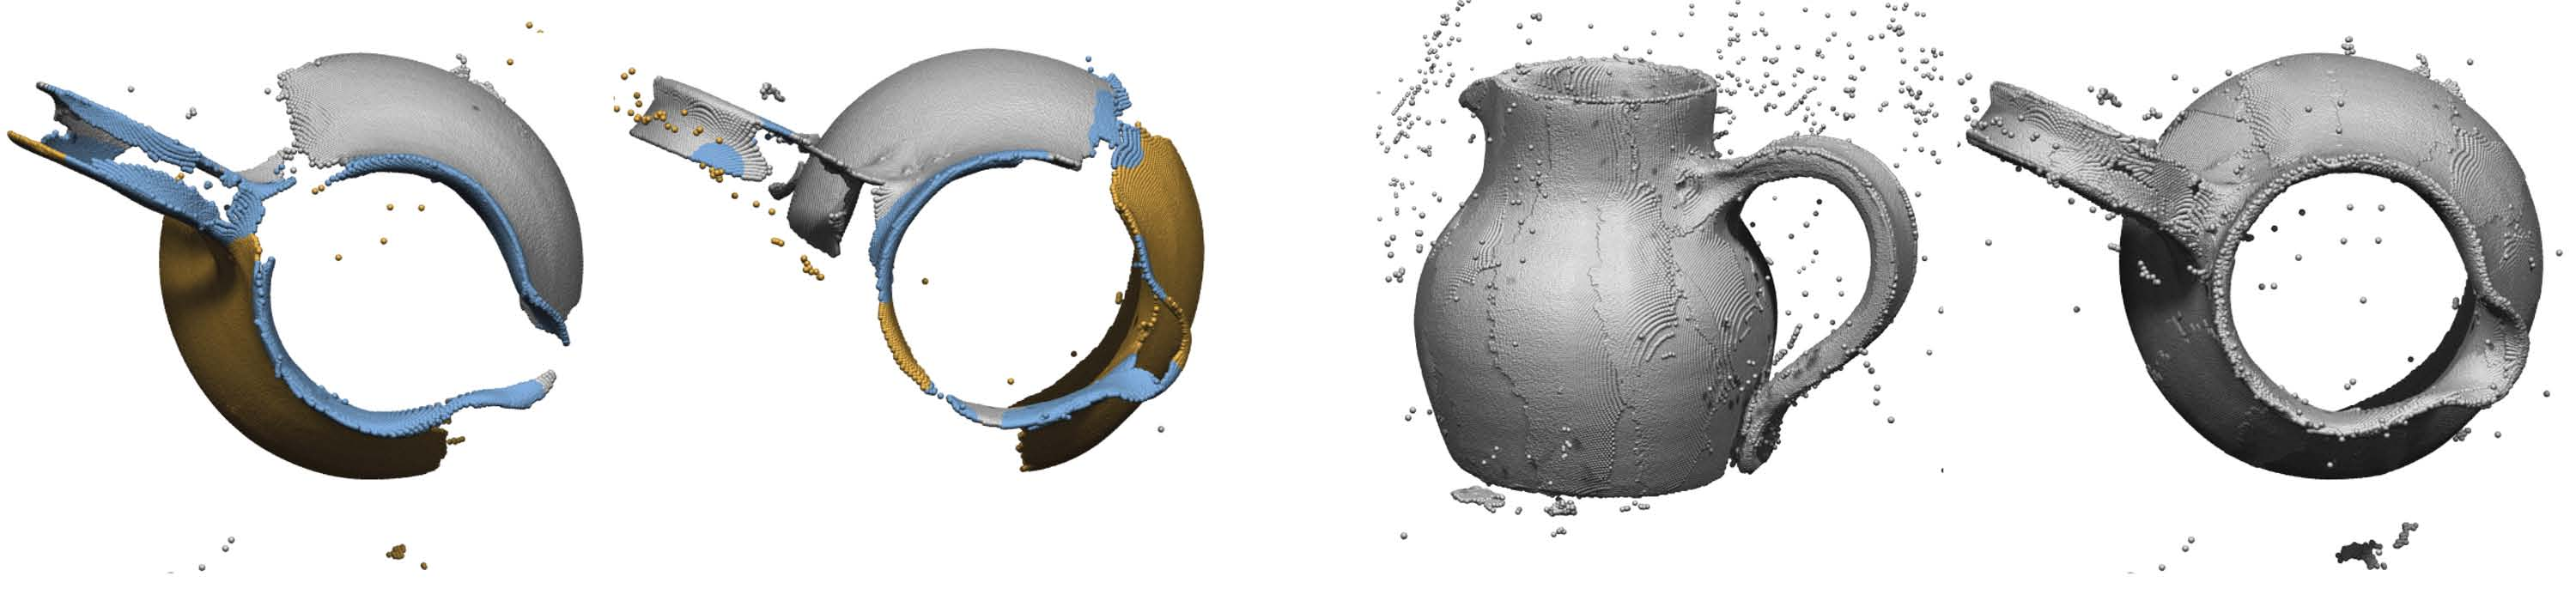
\includegraphics[width=0.99\linewidth]{figures/rigidCMP.jpg}
  \caption{Pairwise alignment of articulated xx. The right is the failure case by [Chang and Zwicker 2009]. \cz{On the coming :)}}
\label{fig:3DRobot}
\end{figure}

For a sequence of partial articulated data, the registration is performed int two main steps.
We first precompute an initial pairwise registration for each pair of consecutive frames, then perform articulated shape reconstruction as in~\cite{Pekelny08}. 
The pairwise registration is addressed as former paragraph.
Segmentation of the scans into rigid parts can readily be done by clustering the transformations obtained from the slippage feature points, 
using the mean shift algorithm~\cite{Comaniciu02}.
This information is used as the input to the second step of articulated shape reconstruction following~\cite{Pekelny08};
this algorithm identifies and tracks the rigid parts in each frame, while accumulating  geometric information over time.
However,~\cite{Pekelny08} requires the user to manually segment each range scan in advance,  whereas we automatically determine  the segmentation.
Figure~\ref{fig:3DHand} shows an articulated hand example.
This synthetic data is generated from a deformation sequence, and the final registered shape is produced from these partial data. 
By using synthetic data, we are able to evaluate the robustness of our reconstruction method using the ground truth, as shown below in Figure~\ref{fig:3DHand}.
Quantitatively, we measured the maximum of the average distance of the reconstruction over all frames as $0.001 D$ where $D$ is the bounding box diagonal length, and
the greatest distance error in any one frame was $0.012 D$.

\begin{figure}[h]
\centering
  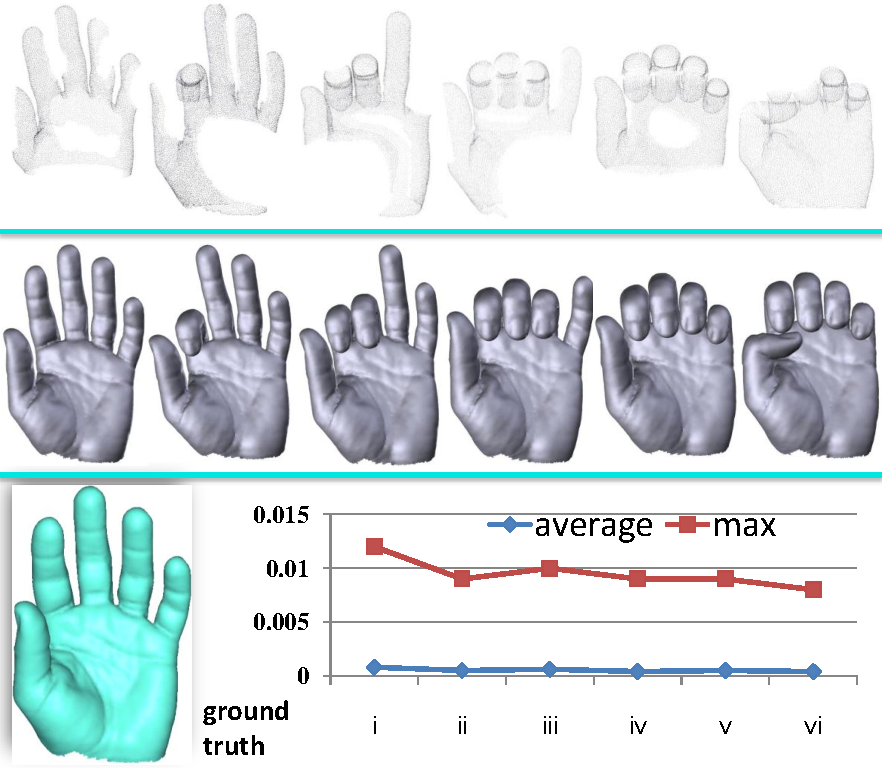
\includegraphics[width=0.95\linewidth]{figures/3DHand.pdf}
  \caption{The registration of articulated hand.
  Above: partial synthetic data with holes is generated from a deformation sequence. 
  The reconstructed meshes are deduced from the registration process (center).
  Below: ground truth shape, and average and maximum distance from the ground truth per frame.}
\label{fig:3DHand}
\end{figure}

%-------------------------------------------------------------------------
\subsection{Deformable surfaces}
\label{subsec:2DDeformable}

Finally, we matched SIFT points showing deforming surfaces\footnote{From \url{http://cvlab.epfl.ch/data/dsr/}}; these showed a cloth and a cushion.
The surface of the cloth underwent relatively smooth deformations, while the surface of the cushion included sharp folds.
This data comes with ground truth, which allows quantitative verification of the accuracy of the matches found.
From each surface set we randomly chose two frames before and after a large deformation.
We randomly chose $100$ corresponding points on each surface to be the features, using the provided ground truth.

We used the above input data as a basis for comparison with the spectral algorithm~\cite{Cour06} (a quadric assignment algorithm),
a third-order tensor algorithm~\cite{Duchenne09},
and the hyper graph matching algorithm~\cite{Zass08}, using the authors' code in each case.
All methods were executed in Matlab on a $2.3$GHz Core2Duo with $2$GB memory.
To enable direct and fair comparison,
~\cite{Duchenne09}, ~\cite{Zass08} and SuperMatching
used the same potential and
all maintained an equivalent tensor size $N$.

In the tests, SuperMatching considered $30000$ feature tuples, while the method of~\cite{Duchenne09} considered 1010000 features  and the method of~\cite{Zass08} used $40000$.
The difference  mainly results from differences in sampling strategy; note that we have the lowest  sampling cost.
The average running time to match two feature sets each with $100$ features was around 8s for SuperMatching, 13s for~\cite{Duchenne09}, 6.5s for~\cite{Zass08}, and 5s for~\cite{Cour06}.
SuperMatching takes less  than the third-order tensor algorithm in~\cite{Duchenne09} as it uses the same tensor size but fewer feature tuples.

Matching accuracy is assessed as the number of correctly matched points (according to the provided ground truth) divided by the total number of points that could potentially be matched.
The results are summarised in Table~\ref{tab:errorrate1} and illustrated in Figure~\ref{fig:2DDeformable}.
Table~\ref{tab:errorrate1} demonstrates that SuperMatching achieves a higher matching accuracy than previous algorithms.
The worst matching result is produced by the spectral quadratic assignment algorithm~\cite{Cour06},
due to the lower discriminatory power of the pairwise geometric constraints used.
Higher-order algorithms perform much better due to the more complex geometric constraints.
Nevertheless, SupeMatching outperforms the third-order algorithm~\cite{Duchenne09} and the hyper graph matching algorithm~\cite{Zass08}, as these do not tale proper advantage of supersymmetry.

%----------------------------------------
%  deformable matching results IMAGES
%----------------------------------------

%----------------------------------------
\begin{figure}[htb]
\centering
  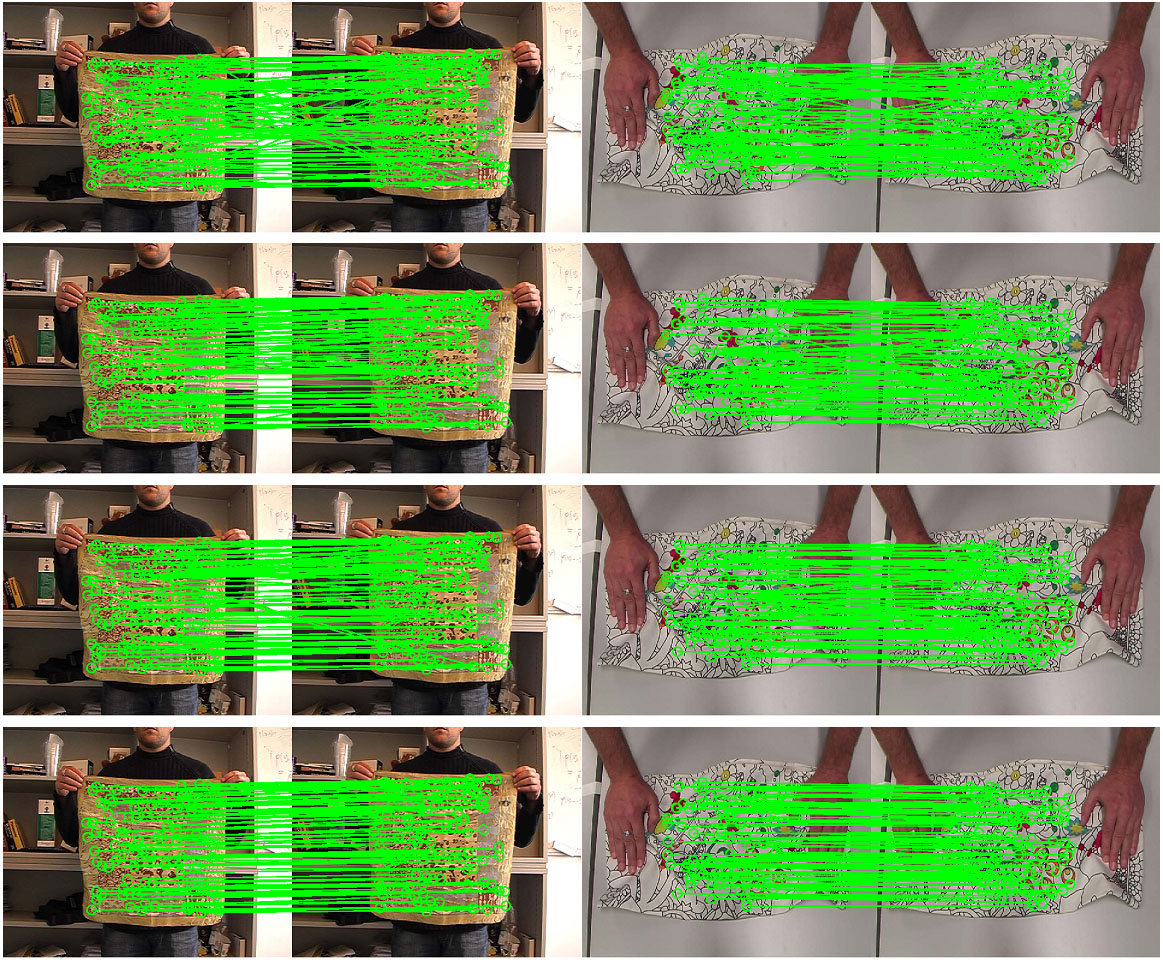
\includegraphics[width=1.00\linewidth]{figures/2DDeformable.jpg}
  \caption{Matching results. Left: cloth set, selected from frame 85 to 110, right: cushion set, selected from frames 144 to 213.
  Top to bottom, spectral method [Cour et al. 2006], hyper graph matching method [Zass and Shashua 2008], a Third-order tensor [Duchenne et al. 2009], and SuperMatching algorithm.}
\label{fig:2DDeformable}
\end{figure}

%----------------------------------------
%  deformable matching results TABLE
%----------------------------------------
\begin{table}[htb]
%\vspace{-4mm}
\centering
%\renewcommand{\arraystretch}{0.8}
\tabcolsep=1pt
\setlength{\aboverulesep}{0pt}
\setlength{\belowrulesep}{0pt}
\caption{Accurate rate of deformable surface matching.}
\hspace{-5ex}
\label{tab:errorrate1}
\small
\begin{tabular}{l|c c c c | c c c c | c c}
\toprule
{Dataset}  & \multicolumn{4}{|c|}{ {cloth}} & \multicolumn{4}{c|}{ {cushion}} & & \\
\hline
 {Matching frames} &  {F80-}	&  {F90-}	& {F95-}	& {F100-} & {F144-} & {F156-}	& {F165-}	& {F172-} & {Feature}	& {Time}  \\
 {}                &  {F90 }    &  {F95 }   & {F100}    & {F105}  & {F156}  & {F165}    & {F172}    & {F188}  & {Tuples}    &  {(s)} \\
\hline
 {SuperMatching}   &  {83\%}    &  {85\%}	& {84\%} 	& {81\%}  & {66\%}	& {60\%}	& {69\%}	& {56\%}  &  {30k}	    &  {8}  \\
%\hline
 {\cite{Zass08}}   & {73\%}	    & {79\%}	& {70\%}	& {72\%}  & {44\%}  & {39\%}    & {54\%}	& {43\%}   & {40k}	    & {6.5}  \\
%\hline
{\cite{Duchenne09}} & {67\%}    & {77\%}    & {73\%}	& {65\%}  & {39\%}	& {31\%}	& {47\%}	& {42\%}   & {1010k}    & {13}  \\
%\hline
 {\cite{Cour06}}   & {27\%}     & {29\%}	&  {22\%}	& {27\%}  & {14\%}  & {5\%}	    & {28\%}	& {7\%}    & {--}       & {5}  \\
\bottomrule
\end{tabular}%
%\vspace{-27pt}
%\vspace{-8mm}
\end{table}%
%
%%%RRM This table would be much better if you showed the percentage of
%%%RRM CORRECT matches, not the percentage of ERRORS.

